\documentclass[../../eatbrain.tex]{subfile}
La home page è da considerare come la vetrina di un negozio fisico, pertanto è indispensabile soddisfare tutte le domande rappresentate dai 6 assi.
\newpage
\subsubsection{Where}
Appena aperto il sito la situazione che mi trovo davanti è la seguente:\\
\begin{figure}[h]
	\centering
	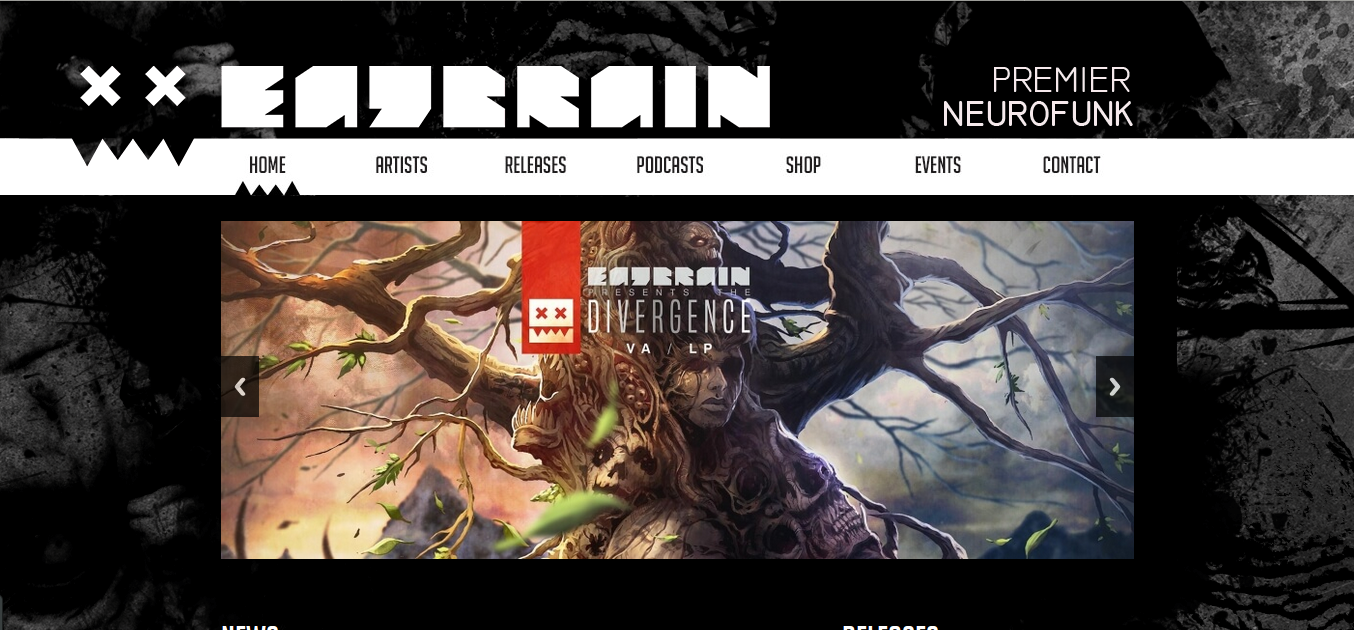
\includegraphics[width=12cm]{immagini/home-visible}
	\label{home-visible}
	\caption{Parte visibile della Home Page una volta aperto il sito}
\end{figure}\\
La risposta a questa domanda è data in modo molto generico: il design suggerisce che si tratti di qualcosa di cupo, le voci del menù fanno pensare a qualcosa di collegato all'ambiente musicale, quasi sicuramente sono entrato in un sito che tratta di musica. Il logo non è il massimo della leggibilità e, considerando i timer limitati dell'utente (in media l'utente dedica 1 minuto e 50 secondi alla scelta del sito ma già dopo 31 secondi iniziano ad affiorare le prime sensazioni negative), impegnare l'utente per decifrare una scritta non risulta certamente la scelta migliore. Lo slogan sulla destra offre un altro indizio: anche se in pochi conoscono il genere Neurofunk, la parola Funk è ben conosciuta globalmente e aiuta ad associare il sito alla musica. \\
La risposta viene raffinata scorrendo verso il basso (ma non tutti gli utenti sono disposti a fare questo sacrificio) dove la panoramica dei contenuti che offre il sito condona la certezza di trovarsi all'interno di un sito musicale, per poi giungere alla fine (footer) dove la breve descrizione dell'etichetta scende in dettaglio sul tipo di musica (\texttt{neurofunk drum\&bass}), ma anche qui una piccola conoscenza preliminare è obbligatoria. \\
\begin{figure}[h]
	\centering
	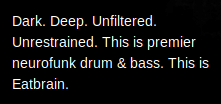
\includegraphics[width=6cm]{immagini/home-why}
	\label{home-where}
	\caption{Specifica del tipo di musica nel footer}
\end{figure}\\
Nel complessivo l'utente potrebbe impiegarci troppo tempo prima di individuare la corretta risposta alla domanda.\\
Per quanto riguarda la domanda "Dove mi trovo nel sito?" la riposta è più immediata: come dicevamo nella sezione \hyperref[sec-nav]{\texttt{Navigazione}} i triangolini nel menù che fanno da breadcrumbs aiutano nell'individuazione, mentre la struttura (slidshow, panoramica di contenuti) è abbastanza simile alle altre home page che si trovano in giro.
\subsubsection{Who}
La riposta anche qui non è immediata, il logo in alto a sinistra (dopo averlo decifrato) mi suggerisce che si tratti di Eatbrain ma per avere una risposta concreta occorre scorrere in fondo alla pagina (anche qui, non tutti gli utenti sono disposti a farlo) fino a raggiungere il footer che mostra delle informazioni più concrete e offre la possibilità di approfondire il discorso visitando le pagine social ad esso collegato.\\
\begin{figure}[h]
	\centering
	
\includegraphics[width=10cm]{immagini/home-who-2}
	\label{img-home-who}
	\caption{Footer che esplicita il who}	
\end{figure}\\
Sebbene i link ai social offrano l'opportunità di ottenere una panoramica completa di chi ospita il sito, possono causare l'abbandono preventivo del portale, che potrebbe giovare alla promozione in generale dell'etichetta, ma sicuramente limita la possibilità che l'utente ritorni nel sito. \\
Un fattore che invece aiuta ulteriormente il Who lo troviamo nell'onnipresenza del logo e della parola Eatbrain all'interno della pagina: quasi tutte le didascalie cominciano con la parola Eatbrain mentre la maggior parte delle immagini presenti nella pagina mostrano il logo piccolo dell'etichetta (le due X con i triangoli in basso che rappresentano una faccia) facilitando l'associazione del logo al chi c'è dietro il sito.
\newpage
\begin{figure}[h]
	\centering
	
\includegraphics[width=12cm]{immagini/logos-everywhere}
	\label{logos-everywhere}
	\caption{Esempi del logo sparsi all'interno della pagina}
\end{figure}
Sostanzialmente una volta entrati all'interno del sito si comprende che la faccia strana è collegata all'immagine dell'azienda e una volta decifrato il logo si capisce che Eatbrain è il fautore del sito.
\subsubsection{Why}
La domanda qui non trova una risposta molto soddisfacente: un primo abbozzo di soluzione lo troviamo nello slogan: "Premier Neurofunk", sono qui per trovare la Neurofunk di qualità migliore; efficace, ma solo se conosco a priori cosa sia questa "Neurofunk".
Come per il Who, la parte sinistra del footer può aiutare con le motivazioni, ma il risultato non è poi così soddisfacente.
\begin{figure}[h]
	\centering
	
\includegraphics[width=5cm]{immagini/slogan}
	\label{home-why}
	\caption{Slogan che risponde allo why}
\end{figure}
\newpage
\subsubsection{What}
La risposta qui è ben rappresentata ma non immediata: come dicevamo nella sezione \hyperref[multimedia]{\texttt{Contenuti Multimediali}} lo slidehow occupa 3/4 della parte visibile della pagina, obbligando l'utente a effettuare lo scroll per ottenere del contenuto significativo dalla pagina. Superando lo sbarramento dello slideshow infatti si ottiene una panoramica di tutte le sezioni presenti nel sito, tramite anteprime o link alle sezioni stesse, soddisfando in pieno la risposta a questa domanda. \\
Il menu iniziale inoltre, offre un assaggio delle sezioni (i titoli) incuriosendo l'utente che potrà trovare soddisfazione nel ottenere un dettaglio maggiore scorrendo la pagina. \\
\begin{figure}[h]
	\centering
	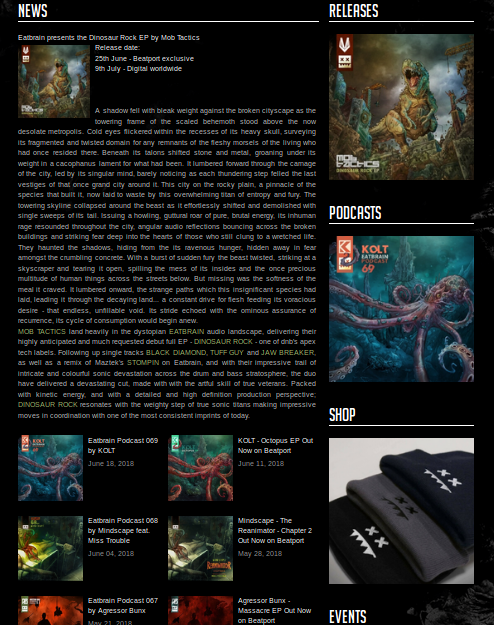
\includegraphics[width=11cm]{immagini/home-what}
	\label{img-home-what}
	\caption{Panoramica delle sezioni nella home page}
\end{figure}
\newpage
\subsubsection{How}
La risposta a questa domanda è la più grande pecca del sito, di solito viene proposta una barra di ricerca per trovare il contenuto desiderato ma in questo caso, anche se il sito non è molto grande, non se ne vede neanche l'ombra. \\
L'unica entità della home page che può rispondere a questa domanda è il menù di navigazione posto in alto che, nonostante la sua semplicità e facilità d'uso, può aumentare i tempi di ricerca dell'utente e peggiorare la sua valutazione della pagina. \\
Tuttavia, come spiegato nella sezione \hyperref[sec-nav]{\texttt{Navigazione}}, con un paio di click l'utente riesce a trovare le informazioni che cerca. \\
Sicuramente poteva essere fatto di più per quanto riguarda questo asse, ad esempio nell'esposizione del contenuto (la panoramica delle sezioni) potevano essere posti dei link per raggiungerle invece che forzare l'utente a tornare in alto ed utilizzare il menù. \\
\begin{figure}[h]
	\centering
	
\includegraphics[width=12cm]{immagini/home-how}
	\label{img-home-how}
	\caption{Menù di navigazione nella home page}
\end{figure}
\subsubsection{When}
La risposta necessita di un leggero impegno da parte dell'utente per essere individuata: nella parte immediatamente visibile della home infatti non ce n'è traccia (lo slideshow come già detto non offre nessuna informazione tangible), per avere un'abbozzo di risposta bisogna scorrere al paragrafo delle News, dove vengono citate alcune date ma senza specificare l'anno. Questa sottigliezza non pone la risposta completa alla domanda che per soddisfarsi necessità di altro tempo per raggiungere la sezione dedicata alle ultime uscite, dove finalmente troviamo la specifica di giorno mese e anno. \\
Ulteriore conferma viene fornita nel footer, dove viene specificato l'anno affianco al copyright. \\
Insomma come già appurato in precedenza: le risposte si trovano ma necessitano sempre di un po' di tempo e ciò, considerati i limitati timer dell'utente, risulta negativo per l'usabilità del sito. \\
\newpage
\begin{figure}[h]
	\centering
	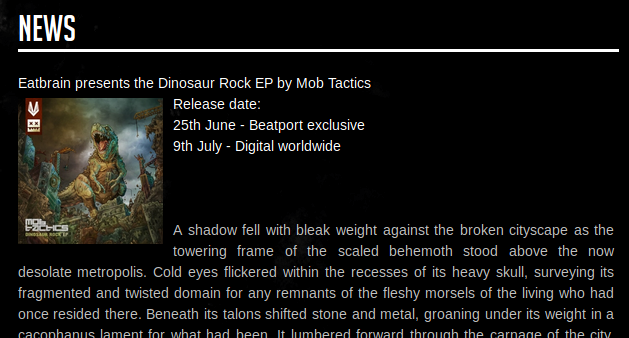
\includegraphics[width=10cm]{immagini/home-when-1}
	\label{home-when-1}
	\caption{Esempio di notizia nella home page}
\end{figure} 
\begin{figure}[h]
	\centering
	
\includegraphics[width=10cm]{immagini/home-when-2}
	\label{home-when-2}
	\caption{Sezione delle ultime uscite nella home page}
\end{figure} 
\newpage
\subsubsection{Considerazioni Generali}
La struttura della home page è ben congeniata rispetto alle aspettative dall'utente ma soffre molto dei problemi citati in precedenza. \\
Il problema più grosso è determinato dallo slideshow, come detto più volte questo occupa 3/4 della pagina visibile e in più ha un tempo di scorrimento troppo lento: ogni immagine rimane 8 secondi e offre un contenuto che meriterebbe al massimo la metà del tempo (non ci sono link, non c'è testo descrittivo, solo immagini). Sapendo che un utente decide la sua permanenza nella pagina in 1 minuto e 50 secondi, il solo aspettare 3 immagini porta via circa 30 secondi (considerando il tempo di caricamento della pagina) e si conclude con un nulla di fatto, lasciando insoddisfatto l'utente. \\
Il contenuto è ben disposto, l'utente semplicemente scorrendo la home page capisce cosa il sito è in grado di offrire; ma come viene fatta una panoramica dei contenuti, la home page offre anche una panoramica di tutti gli errori descritti nella sezione \hyperref[convenzioni]{\texttt{Rispetto delle Convenzioni}}.
Altra nota negativa che non traspare dalla valutazione dei 6 assi è la piccolezza trascurata nella vetrina delle ultime release: la colonna di destra presenta dei link che accompagnano l'utente al di fuori della pagina e conducono al sito di Beatport, dove poter acquistare la traccia indicata. Purtroppo da nessuna parte viene indicato che cliccando il link si uscirà dal sito, comportamento che può lasciare disorientato l'utente. \\
In generale la Home Page si presenta come una buona vetrina, pur tralasciando alcune sottigliezze che possono peggiorare l'esperienza dell'utente.